\documentclass[11pt]{article}
\usepackage[margin=1in]{geometry}
\usepackage[T1]{fontenc}
\usepackage[utf8]{inputenc}
\usepackage{amsmath,amssymb,mathtools}
\usepackage{booktabs}
\usepackage{array}
\usepackage{graphicx}
\usepackage{float}
\usepackage{caption}
\usepackage{enumitem}
\usepackage[section]{placeins}
\usepackage{xcolor}
\usepackage{hyperref}

\hypersetup{
  colorlinks=true,
  linkcolor=blue!45!black,
  urlcolor=blue!45!black,
  citecolor=blue!45!black
}

\setlength{\parindent}{0pt}
\setlength{\parskip}{0.55em}
\setlist[itemize]{leftmargin=1.4em,itemsep=0.2em,topsep=0.2em}
\setlist[enumerate]{leftmargin=1.6em,itemsep=0.25em,topsep=0.25em}
\captionsetup{font=small,labelfont=bf}
\sloppy

\newcommand{\R}{\mathbb{R}}
\newcommand{\Prb}{\mathbb{P}}
\newcommand{\1}{\mathbf{1}}
\newcommand{\Ball}{B}
\newcommand{\vol}{\operatorname{vol}}

\title{\vspace{-1.2em}Testing Stratified Manifold Hypothesis in Vision}
\author{}
\date{Revised July 30, 2026}

\begin{document}
\maketitle

\begin{abstract}
We begin with a global topological hypothesis for vision representations: for
every token embedding $t$ in the representation support $\mathcal E$, there is
a radius $r_\ast(t)$ for which the local neighborhood of $t$ is homeomorphic to
an intrinsic Euclidean space $\R^{d(t)}$. This statement is topological and is
not directly amenable to finite-sample testing. We therefore study a stronger,
testable local surrogate: after conditioning on the neighborhood, probability
mass is approximately uniform with respect to intrinsic volume. This assumption
determines the probability mass of every concentric shell around $t$. In
particular, the log-radius $Z=\log(r_\ast/\|X-t\|_2)$ follows an exponential
distribution with unknown rate $d(t)$. We test this necessary radial signature
with a fitted-scale Anderson--Darling statistic and analytic finite-sample
critical values. Controlled simulations recover the nominal false positive
rate and show increasing power against inner- and outer-heavy alternatives. We
also report patch-level ImageNet experiments and experiments with two released
visual-token generators: raster-order LlamaGen and next-scale VAR. The
cross-pipeline results expose substantial tokenizer dependence and show that
codebook rejection alone does not reliably predict generator uncertainty.
Taken together, the experiments reject a universal locally homogeneous
manifold model for vision tokens. They are compatible with, but do not by
themselves establish, a stratified organization of representation space.
\end{abstract}

\section{Global Hypothesis and Testable Surrogate}

Let $\mathcal E\subseteq\R^{D_{\mathrm{amb}}}$ denote the support of an
embedding distribution, and let $t\in\mathcal E$ be an anchor token, image patch
embedding, transformer state, or VQ codebook vector. The ambient embedding
dimension is $D_{\mathrm{amb}}$, whereas $d(t)\le D_{\mathrm{amb}}$ denotes the
intrinsic dimension near $t$. A precise version of the global local-Euclidean
hypothesis is
\begin{equation}
  \mathcal H_{\mathrm{top}}:\qquad
  \forall t\in\mathcal E,\quad
  \exists\ r_\ast(t)>0,\ d(t)\in\{1,\ldots,D_{\mathrm{amb}}\}
  \quad\text{such that}\quad
  \mathcal E\cap \Ball^\circ_{D_{\mathrm{amb}}}(t,r_\ast(t))
  \cong \R^{d(t)}.
  \label{eq:topological-hypothesis}
\end{equation}
Here $\cong$ denotes homeomorphism and $\Ball^\circ$ is an open ambient ball.
The use of an open ball matters: an open $d$-ball is homeomorphic to $\R^d$,
whereas a closed ball is compact and cannot be homeomorphic to $\R^d$. For a
stratified support, Equation~\eqref{eq:topological-hypothesis} can be applied to
the stratum containing $t$; tokens near a boundary or an intersection of strata
need not admit one regular local chart.

The topological hypothesis alone does not determine a probability law. A
homeomorphism preserves continuity and open sets, but it need not preserve
Euclidean distances, volumes, or sampling density. Statistical testing
therefore requires an additional localized measure hypothesis. At a scale where
the chart is well approximated by its tangent geometry, we use
\begin{equation}
  \mathcal H_{0,t}(d):\qquad
  X\mid \{X\in\mathcal E,\ \|X-t\|_2<r_\ast(t)\}
  \ \text{is uniform with respect to local $d$-dimensional volume.}
  \label{eq:localized-null}
\end{equation}
Operationally, Equation~\eqref{eq:localized-null} approximates the neighborhood
by a uniform tangent ball $\Ball_d(t,r_\ast)$. It adds local metric regularity
and approximately constant sampling density to the purely topological claim.
Consequently it is a stronger assumption: rejecting it does not, by itself,
disprove the existence of a homeomorphism.

Choose radii
\[
  0<r_1<r_2<\cdots<r_K=r_\ast
\]
and consider the nested neighborhoods
\[
  \Ball(t,r_1)\subset\Ball(t,r_2)\subset\cdots\subset\Ball(t,r_\ast).
\]
The localized question is whether conditional probability mass near $t$ grows
with radius as it would in this smooth, uniformly sampled $d$-dimensional
region. The alternative includes boundaries, intersections of strata, mixed
visual modes, nonuniform density, strong curvature at scale $r_\ast$, and local
geometry that cannot be represented by one effective dimension.

A rejection means that the observed radial mass growth is inconsistent with
the smooth-volume model at the selected scale. It does not by itself identify
which geometric or sampling effect caused the departure.

\section{The Radial Volume Law}

Write
\[
  R=\|X-t\|_2.
\]
The volume of a $d$-dimensional ball of radius $r$ is $c_d r^d$, where $c_d$
depends only on $d$. Uniformity in the outer ball gives, for
$0\le r\le r_\ast$,
\begin{align}
  F_d(r)
  &=\Prb_{\mathcal H_{0,t}(d)}(R\le r) \\
  &=\frac{\vol(\Ball_d(t,r))}{\vol(\Ball_d(t,r_\ast))} \\
  &=\frac{c_d r^d}{c_d r_\ast^d}
    =\left(\frac{r}{r_\ast}\right)^d.
  \label{eq:radial-cdf}
\end{align}
The constant $c_d$ cancels. Only the intrinsic dimension and the normalized
radius remain.

The same formula gives the probability mass function over concentric shells.
Set $r_0=0$, define
\[
  A_k(t)=\{x\in\mathcal E:r_{k-1}<\|x-t\|_2\le r_k\},
\]
and let the discrete shell index $S$ equal $k$ when $X\in A_k(t)$. Under the
localized null, its conditional PMF is
\begin{equation}
  q_k(d)
  :=\Prb(S=k\mid R\le r_\ast)
  =\frac{r_k^d-r_{k-1}^d}{r_\ast^d},
  \qquad k=1,\ldots,K.
  \label{eq:shell-pmf}
\end{equation}
Thus ``uniform on shells'' does not generally mean equal probability for
equal-width shells: outer shells have more volume. It means that shell mass is
proportional to $d$-dimensional shell volume.

If $p_{t,k}=\Prb(S=k\mid R\le r_\ast)$ denotes the true shell PMF, one precise
meaning of ``close'' at shell resolution $K$ is
\begin{equation}
  \Delta_{\mathrm{shell}}(t;d)
  =\frac12\sum_{k=1}^K\left|p_{t,k}-q_k(d)\right|
  \le \varepsilon,
  \label{eq:shell-closeness}
\end{equation}
for a scientifically chosen tolerance $\varepsilon$. The exact reference null
sets $\varepsilon=0$. The statistic used below avoids fixing shell boundaries
and tests the corresponding continuous radial law.

For visualization, the radii
\[
  r_k=r_\ast\left(\frac{k}{K}\right)^{1/d}
\]
define equal-volume shells and reduce Equation~\eqref{eq:shell-pmf} to
$q_k(d)=1/K$. Their histograms help show whether a
departure is concentrated near the anchor, near the boundary, or at an
intermediate radius. The formal statistic below uses the unbinned radii.

\section{The Log-Radius Transformation}

Define
\[
  Z=\log\frac{r_\ast}{R},
  \qquad Z\ge0.
\]
For any $z\ge0$,
\begin{align}
  \Prb(Z>z)
  &=\Prb\left(\log\frac{r_\ast}{R}>z\right) \\
  &=\Prb\left(R<r_\ast e^{-z}\right) \\
  &=\left(\frac{r_\ast e^{-z}}{r_\ast}\right)^d
    =e^{-dz}.
\end{align}
Therefore
\[
  \mathcal H_{0,t}(d)\quad\Longrightarrow\quad
  Z\sim\operatorname{Exp}(d),
  \label{eq:exponential}
\]
where $d$ is the rate and $1/d$ is the mean.

This transformation is intuitive. A point close to the outer boundary has
$Z\approx0$, while a point unusually close to the anchor has a large value of
$Z$. Under smooth $d$-dimensional volume growth, these log-radii must have the
shape of an exponential distribution. Changing $d$ only stretches or
compresses their scale.

\section{Estimating Dimension}

For log-radii $Z_1,\ldots,Z_N$, the exponential log objective is
\[
  \ell(d)=N\log d-d\sum_{i=1}^N Z_i.
\]
Differentiation gives
\[
  \frac{\partial\ell}{\partial d}
  =\frac{N}{d}-\sum_{i=1}^N Z_i,
\]
so the fitted local dimension is
\[
  \widehat d
  =\frac{N}{\sum_{i=1}^N Z_i}
  =\frac{1}{\overline Z}
  =\frac{N}{\sum_{i=1}^N\log(r_\ast/R_i)}.
  \label{eq:dhat}
\]
This is the same radial dimension estimator obtained directly from the ball
volume density.

To remove the unknown scale from the shape test, define
\[
  V_i=\frac{Z_i}{\overline Z}=\widehat d Z_i.
\]
If the null is correct, the $V_i$ should follow the fitted unit-rate
exponential CDF
\[
  H(v)=1-e^{-v},\qquad v\ge0.
\]

\section{Test Statistic and Decision Rule}

Let $V_{(1)}\le\cdots\le V_{(N)}$ be the ordered standardized log-radii. We use
the Anderson--Darling statistic
\[
  A_N^2
  =-N-\frac{1}{N}\sum_{i=1}^N(2i-1)
  \left[
    \log H(V_{(i)})
    +\log\bigl(1-H(V_{(N+1-i)})\bigr)
  \right].
  \label{eq:ad}
\]
Large values mean that the empirical log-radius distribution is inconsistent
with a single exponential shape.

The statistic weights discrepancies by
$[H(v)(1-H(v))]^{-1}$, so deviations near both tails matter. This is useful for
local geometry: the lower tail corresponds to points crowded near the outer
radius, while the upper tail corresponds to points unusually close to the
anchor. The statistic is also invariant to a common rescaling of all $Z_i$,
which is why the unknown dimension can be fitted without changing the basic
decision rule.

For an exponential distribution with fitted scale, standard finite-sample
critical values are
\[
  c_N(\alpha)=\frac{a_\alpha}{1+0.6/N},
\]
with
\begin{center}
\begin{tabular}{c@{\qquad}ccccc}
\toprule
$\alpha$ & 0.15 & 0.10 & 0.05 & 0.025 & 0.01 \\
\midrule
$a_\alpha$ & 0.922 & 1.078 & 1.341 & 1.606 & 1.957 \\
\bottomrule
\end{tabular}
\end{center}
At level $\alpha$, reject when
\[
  A_N^2>c_N(\alpha).
  \label{eq:decision}
\]
The experiments use $\alpha=0.05$. For visualization we report the normalized
score $S_N=A_N^2/c_N(0.05)$, so the rejection threshold is always $S_N=1$.

\section{Adaptive Outer Radius}

In nearest-neighbor experiments, $r_\ast$ is the distance to the outer retained
neighbor. That neighbor lies exactly on the selected boundary and therefore
has a deterministic log-radius of zero. We use it only to define $r_\ast$ and
exclude it from the statistic. Conditional on the selected outer radius, the
remaining inner radii follow Equation~\eqref{eq:radial-cdf} under the local
null. Thus a neighborhood of 96 distances contributes 95 tested log-radii, and
a neighborhood of 128 distances contributes 127.

For each anchor $t$, the complete procedure is:
\begin{enumerate}
  \item Select $M$ nearest neighbors and set $r_\ast$ to the distance of the
  $M$th neighbor.
  \item Remove the boundary-defining neighbor and compute
  $Z_i=\log(r_\ast/R_i)$ for the remaining $N=M-1$ points.
  \item Estimate $\widehat d=1/\overline Z$ and form
  $V_i=Z_i/\overline Z$.
  \item Compute $A_N^2$ from Equation~\eqref{eq:ad}.
  \item Reject when $A_N^2>c_N(\alpha)$.
  \item Correct across many anchors, for example with a false discovery rate
  procedure if a global discovery claim is required.
\end{enumerate}

The neighborhood size controls a bias--variance tradeoff. Small neighborhoods
are more local but noisier. Large neighborhoods improve precision but can mix
strata or encounter curvature. Results should therefore be checked over
several neighborhood sizes.

\section{Synthetic Size and Power Experiment}

We evaluate the analytic decision rule in a controlled setting with $d=4$.
Each configuration uses 5,000 independent trials. Under the null, the enclosed
volume $U=R^4$ is uniform on $[0,1]$. The alternatives replace this law with
$U\sim\operatorname{Beta}(0.45,1.60)$ for inner-heavy mass and
$U\sim\operatorname{Beta}(1.60,0.45)$ for outer-heavy mass. These alternatives
change the radial shape rather than merely changing the effective dimension.

\begin{table}[H]
\centering
\small
\caption{Synthetic size and power of the analytic log-radius test.}
\begin{tabular}{rrrrrr}
\toprule
$N$ & Critical $A_N^2$ & Null reject & Inner reject & Outer reject & Mean null $A_N^2$ \\
\midrule
64  & 1.3285 & 0.0510 & 0.4754 & 0.9974 & 0.5894 \\
128 & 1.3347 & 0.0532 & 0.8214 & 1.0000 & 0.5985 \\
256 & 1.3379 & 0.0456 & 0.9912 & 1.0000 & 0.5921 \\
512 & 1.3394 & 0.0452 & 1.0000 & 1.0000 & 0.5914 \\
\bottomrule
\end{tabular}
\label{tab:synthetic}
\end{table}

The null rejection rate ranges from $4.52\%$ to $5.32\%$, close to the target
$\alpha=0.05$. At $N=64$, power is $47.54\%$ against the inner-heavy
alternative and $99.74\%$ against the outer-heavy alternative. Inner-heavy
power rises to $99.12\%$ by $N=256$.

\section{ImageNet Patch-Level Experiment}

We apply the analytic log-radius test to 16 images from the ImageNet validation
set. Each image is resized to $224\times224$ and decomposed into a
$14\times14$ grid of $16\times16$ patches. A patch is represented by a
downsampled RGB feature vector. For each of 3,136 patch anchors, we use 96
nearest patch features. The outer distance defines $r_\ast$, leaving 95
log-radii for the statistic.

\begin{table}[H]
\centering
\small
\caption{ImageNet patch-level exponentiality experiment.}
\begin{tabular}{lr}
\toprule
Quantity & Value \\
\midrule
Validation images & 16 \\
Patch anchors & 3136 \\
Patch size & $16\times16$ \\
Nearest neighbors & 96 \\
Tested inner radii & 95 \\
Critical $A_N^2$ at $\alpha=0.05$ & 1.3326 \\
Rejected anchors & 1396 \\
Rejection fraction & 0.4452 \\
Mean fitted dimension & 6.4631 \\
Median fitted dimension & 5.7461 \\
Median $A_N^2$ & 1.1503 \\
\bottomrule
\end{tabular}
\label{tab:imagenet}
\end{table}

The test rejects the local smooth-volume null for $44.52\%$ of patch anchors.
The heatmaps in Figure~\ref{fig:heatmaps} localize the departures. They are maps
of radial model mismatch, not ground-truth singularity labels. Texture
repetition, object boundaries, background transitions, and the simple RGB
feature representation can all contribute.

\begin{figure}[p]
\centering
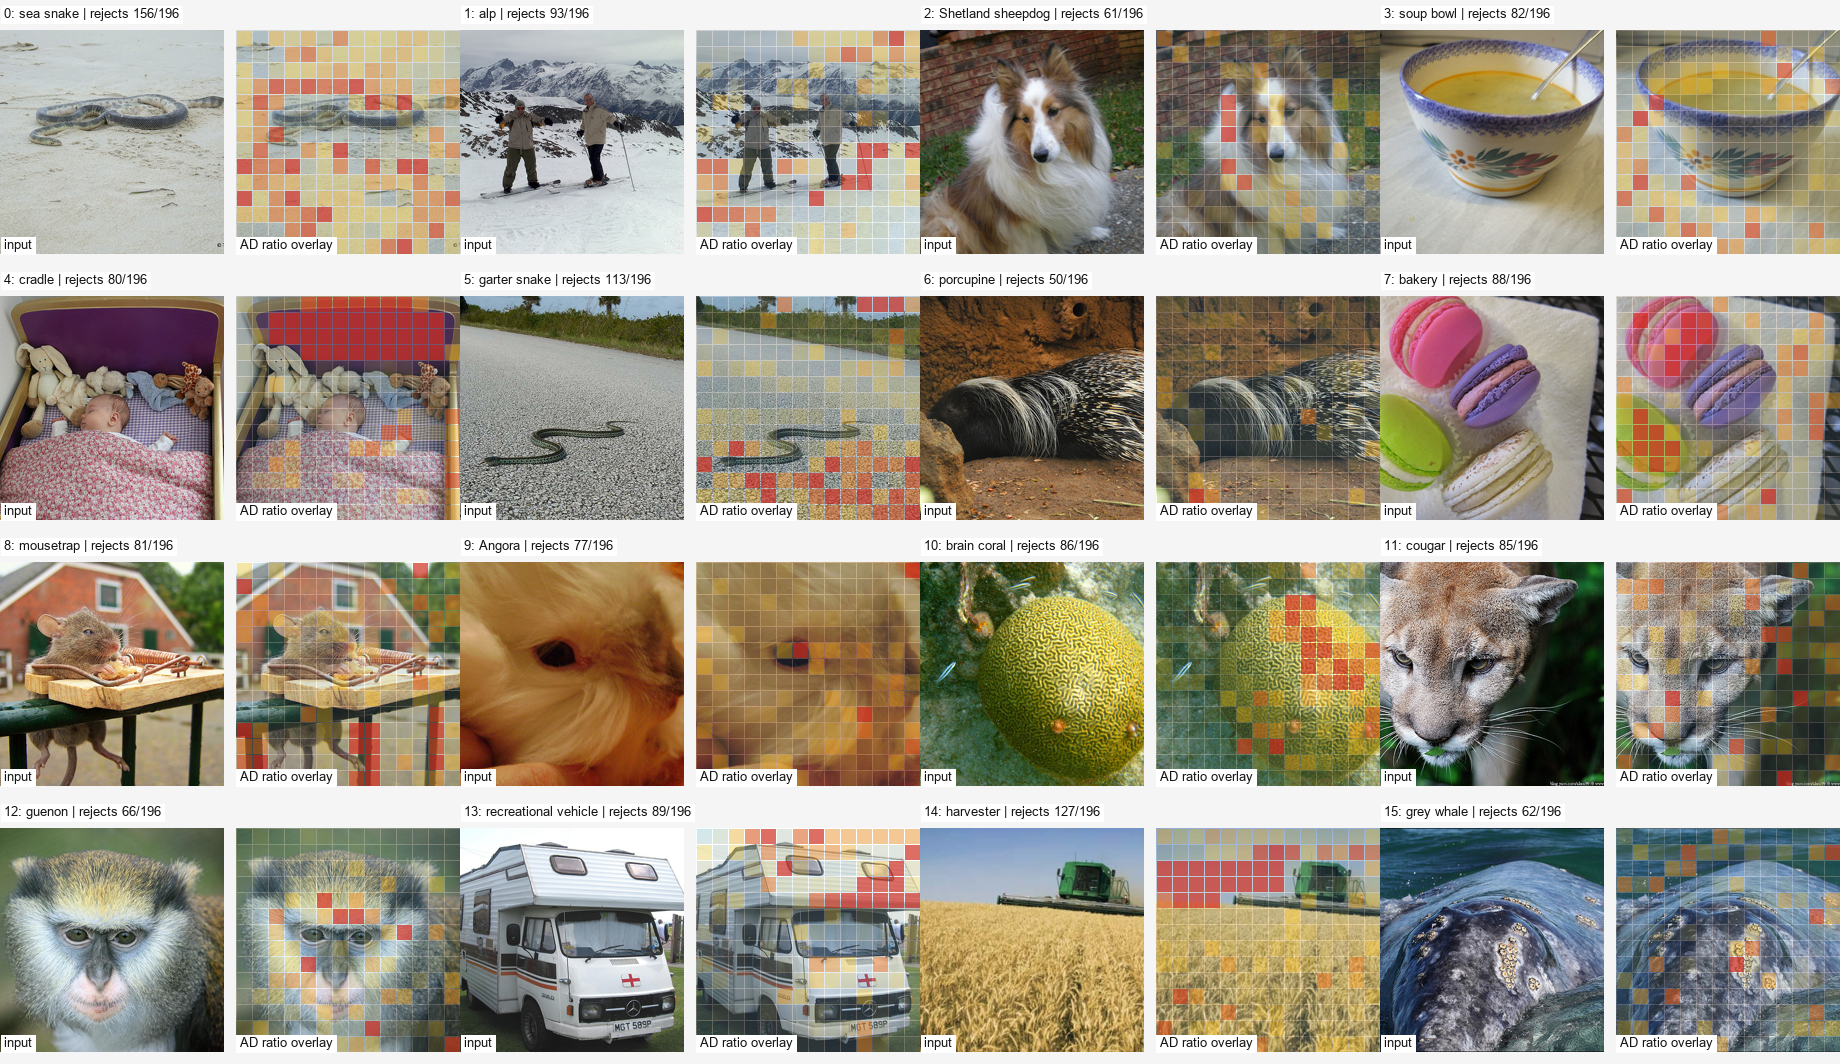
\includegraphics[width=0.95\linewidth]{images/imagenet_shell_heatmap_gallery.png}
\caption{ImageNet validation images with patch-level normalized
Anderson--Darling score overlays. Warmer regions indicate stronger departures;
the analytic rejection threshold is a score of one.}
\label{fig:heatmaps}
\end{figure}

\begin{figure}[p]
\centering
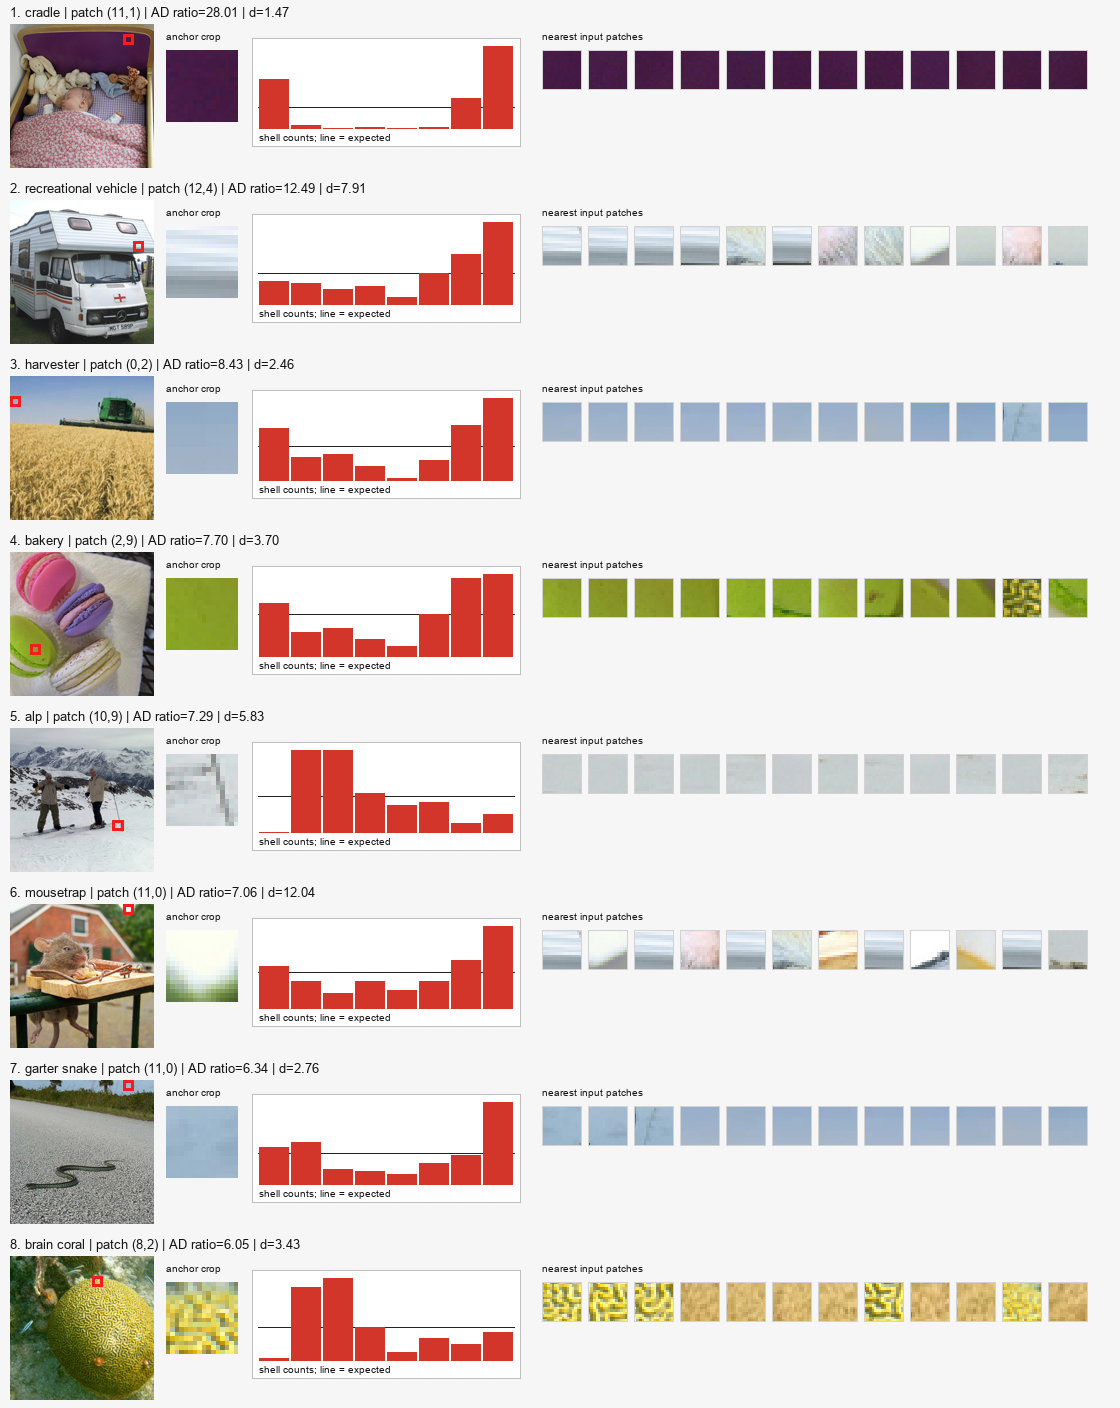
\includegraphics[width=0.95\linewidth]{images/imagenet_shell_anchor_examples.png}
\caption{Representative rejected patch anchors. Annulus histograms are
descriptive views of the radial mismatch; the formal decision uses the
unbinned log-radii. Nearest patches show the local feature neighborhood.}
\label{fig:anchors}
\end{figure}

\section{VQ Tokenizer and GPT-Style Vision Generator}

We next analyze a matched FoundationVision/LlamaGen pipeline
\cite{sun2024llamagen} containing a
pretrained VQ tokenizer and a GPT-style autoregressive transformer over VQ code
IDs. The VQ codebook has 16,384 vectors in an 8-dimensional embedding table.
For every code, we use 128 nearest codebook neighbors, define $r_\ast$ with the
outer neighbor, and apply the statistic to the remaining 127 log-radii. We then
join code-level decisions to 16,384 ImageNet validation positions encoded by
the same tokenizer and evaluated by the matched autoregressive model.

A finite VQ codebook is not literally a positive-dimensional manifold. With
the topology induced from Euclidean space, a finite set of distinct vectors is
discrete and therefore cannot be homeomorphic to an open subset of $\R^d$ for
$d>0$. The codebook experiment instead treats learned prototypes as a finite
geometric proxy for an underlying latent support. Its rejection rate measures
whether local prototype spacing follows smooth-volume growth; it is not a
literal estimate of the fraction of topologically singular points.

\begin{table}[H]
\centering
\small
\caption{VQ/GPT-style log-radius exponentiality experiment.}
\begin{tabular}{lr}
\toprule
Quantity & Value \\
\midrule
VQ codebook size & 16384 \\
Nearest neighbors per code & 128 \\
Tested inner radii & 127 \\
Critical $A_N^2$ at $\alpha=0.05$ & 1.3347 \\
Rejected VQ codes & 16247 \\
Codebook rejection fraction & 0.9916 \\
Mean fitted codebook dimension & 6.5448 \\
Median fitted codebook dimension & 6.5211 \\
Large-fiber rejection rate & 0.9919 \\
Rest-code rejection rate & 0.9916 \\
ImageNet AR positions joined & 16384 \\
Positions using rejected target codes & 0.9847 \\
Rejected-target branch-KS shift & $-0.3605$ \\
Rejected-target branch-entropy shift & $+0.3146$ \\
\bottomrule
\end{tabular}
\label{tab:vqgpt}
\end{table}

The test rejects the local volume law for $99.16\%$ of VQ codebook vectors.
This high rate is plausible for a learned quantization codebook: its vectors
are optimized for reconstruction and token usage, not sampled uniformly from a
smooth chart. It should be interpreted as strong model mismatch, not as a
literal estimate of the fraction of geometrically singular codes.

ImageNet target positions using rejected VQ codes have lower autoregressive
branch KS by $0.3605$ and higher normalized branch entropy by $0.3146$ than the
remaining positions; both permutation p-values are approximately
$2\times10^{-4}$. Only 250 joined positions use non-rejected codes, so these
conditional differences should be treated as exploratory. The paired decoding
experiment remains more selective: a flatness-ranked singular set increases
decoded crop diversity by $0.00452$, with $23/32$ paired wins and a one-sided
sign-flip p-value of $4.0\times10^{-5}$.

\begin{figure}[p]
\centering
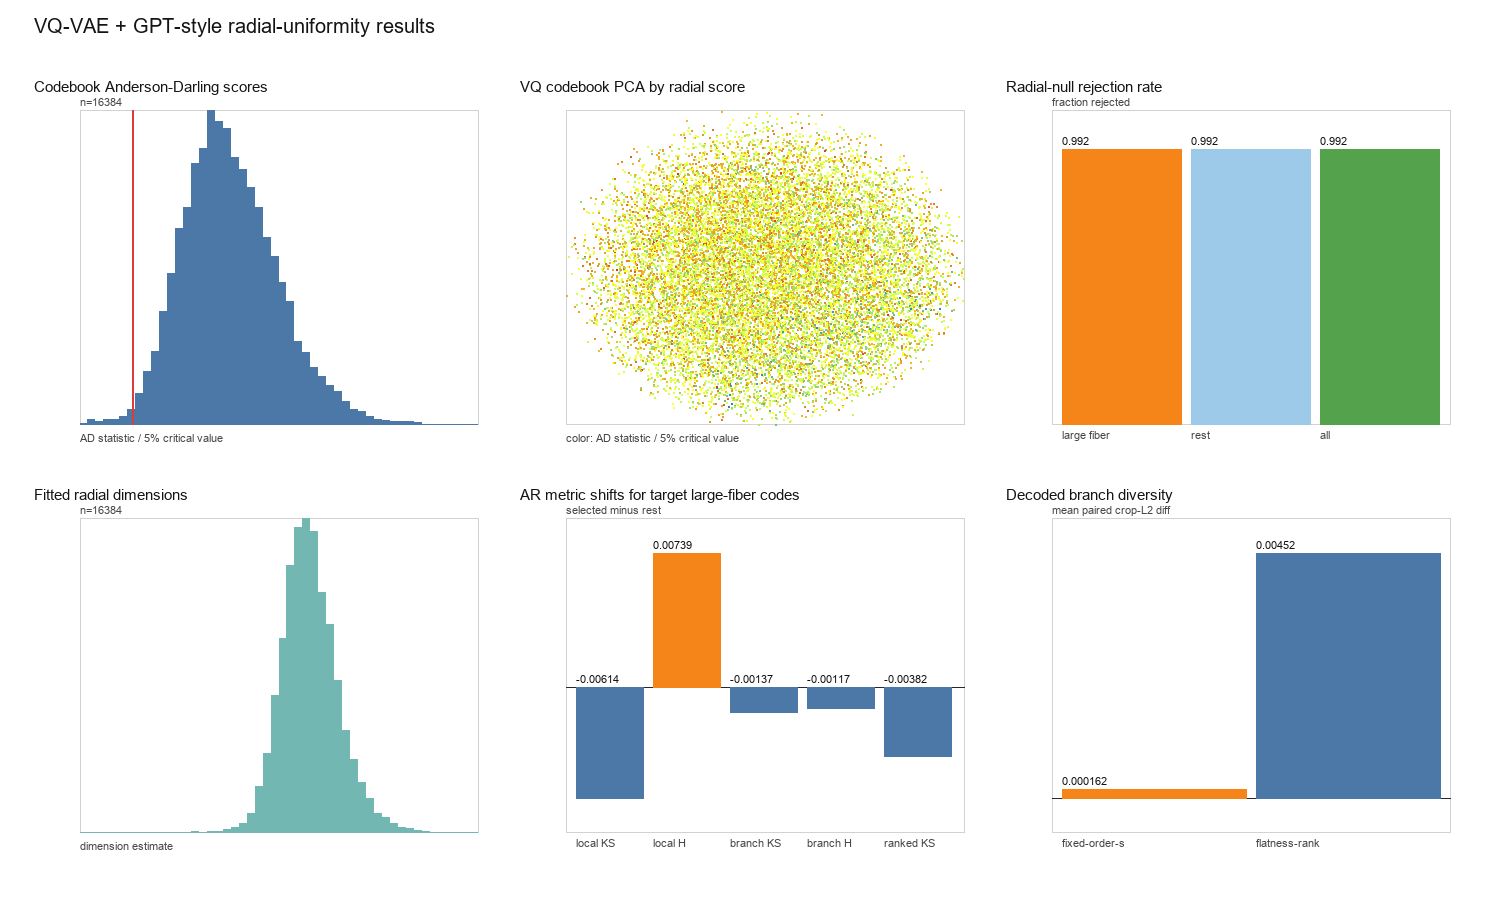
\includegraphics[width=0.95\linewidth]{images/vq_gpt_shell_dashboard.png}
\caption{VQ tokenizer and GPT-style generator results. Panels show normalized
Anderson--Darling scores, codebook geometry, rejection rates, fitted
dimensions, autoregressive metric shifts, and paired decoded branch diversity.}
\label{fig:vqgpt-dashboard}
\end{figure}

\begin{figure}[p]
\centering
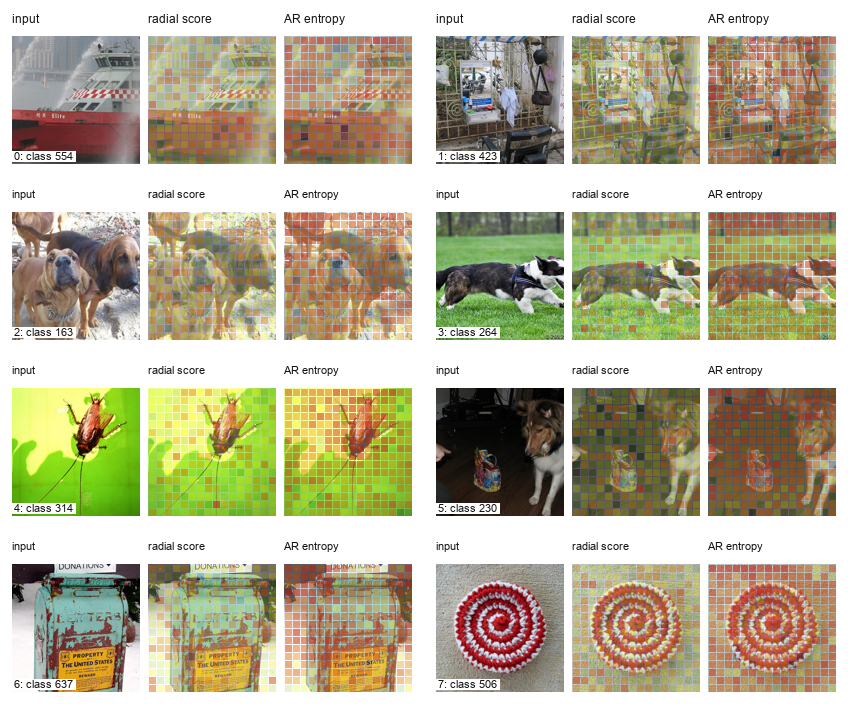
\includegraphics[width=0.95\linewidth]{images/vq_gpt_imagenet_shell_heatmap_gallery.png}
\caption{ImageNet examples under the matched VQ tokenizer and autoregressive
model. Each row shows the input, the normalized log-radius test score of the
target VQ code, and the local autoregressive branch entropy.}
\label{fig:vqgpt-heatmaps}
\end{figure}

\section{Next-Scale Visual Autoregression with VAR}

To test whether the preceding behavior is specific to raster-order generation,
we repeat the experiment with Visual Autoregressive Modeling (VAR)
\cite{tian2024var}. VAR represents an image by a sequence of discrete token
maps at progressively finer spatial scales and predicts the next scale rather
than the next token in raster order. We evaluate the released VAR-d16 and
VAR-d30 class-conditional generators. Their reported parameter counts are
$310$ million and $2.0$ billion, and their reported ImageNet $256\times256$
FID values are $3.55$ and $1.97$, respectively; these benchmark FIDs are model
metadata and were not recomputed in our experiment.

Both generators use the same released VQ-VAE. Its codebook contains $4096$
vectors in $\R^{32}$. Because code-vector norm is a learned nuisance scale, we
first map every nonzero code $e_j$ to $e_j/\lVert e_j\rVert_2$ and then measure
Euclidean distances. For each anchor code, we retain its $128$ nearest distinct
codes, set $r_\ast$ to the farthest retained distance, and apply the fitted-scale
Anderson--Darling test to the remaining $127$ log-radii. At level $0.05$, with
critical value $1.3347$, the test rejects $1118$ of $4096$ anchors, or
$27.29\%$. The fitted local dimension has mean $27.42$ and median $28.83$.
Thus the same test that rejects $99.16\%$ of normalized LlamaGen codes rejects
only $27.29\%$ of normalized VAR codes. Radial codebook geometry is therefore
strongly dependent on tokenizer design and parameterization.

We next ask whether rejected target codes coincide with less concentrated
generator predictions. For each model depth, we teacher-force $16$ ImageNet
validation images and $16$ newly generated class-conditional images through
all scales, producing $4096$ final-scale positions in each group. At every
position we record whether its target code is rejected by the codebook test.
We also record two summaries of the generator's $32$ highest-probability next
codes: (i) a branch KS distance from the uniform CDF, where smaller values mean
a flatter branch, and (ii) normalized branch entropy, where larger values mean
a flatter branch.

Inference is clustered at the image level. Within each image, we compute the
difference between positions whose target code is rejected and the remaining
positions. We then average the $16$ paired image differences and obtain a
one-sided exact sign-flip p-value by enumerating all $2^{16}$ image-level sign
assignments. This preserves the image as the independent sampling unit instead
of treating spatial positions as independent observations.

\begin{table}[H]
\centering
\small
\caption{VAR codebook and teacher-forced generator experiments. A negative
$\Delta\mathrm{KS}$ or positive $\Delta H$ is the predicted flatter-branch
direction. P-values are exact one-sided image-level sign-flip tests.}
\resizebox{0.95\linewidth}{!}{%
\begin{tabular}{lrr}
\toprule
Quantity & VAR-d16 & VAR-d30 \\
\midrule
Parameters & 310M & 2.0B \\
Reported ImageNet FID & 3.55 & 1.97 \\
Shared normalized-codebook rejection & 0.2729 & 0.2729 \\
\midrule
ImageNet images / positions & 16 / 4096 & 16 / 4096 \\
Rejected-target fraction & 0.3052 & 0.3052 \\
$\Delta\mathrm{KS}$; p-value & $-0.00232$; 0.1889 & $+0.00199$; 0.7370 \\
$\Delta H$; p-value & $+0.00224$; 0.0995 & $-0.00179$; 0.7506 \\
\midrule
Generated images / positions & 16 / 4096 & 16 / 4096 \\
Rejected-target fraction & 0.2834 & 0.2883 \\
$\Delta\mathrm{KS}$; p-value & $-0.00125$; 0.3490 & $-0.00050$; 0.4403 \\
$\Delta H$; p-value & $+0.00100$; 0.3353 & $-0.00076$; 0.6136 \\
\bottomrule
\end{tabular}%
}
\label{tab:var}
\end{table}

None of the four model--image-group comparisons gives reliable image-level
evidence in the predicted direction. VAR-d16 on real ImageNet has the largest
entropy shift, but its one-sided p-value is $0.0995$; the other p-values are
larger. Increasing generator depth from d16 to d30 does not strengthen the
association. The experiment therefore separates two claims that should not be
conflated: the shell test measures radial organization of the tokenizer's
codebook, whereas branch entropy and branch KS measure uncertainty in the
conditional generator. A geometric mismatch in the former is not, by itself,
evidence of polysemy or branching in the latter.

\begin{figure}[p]
\centering
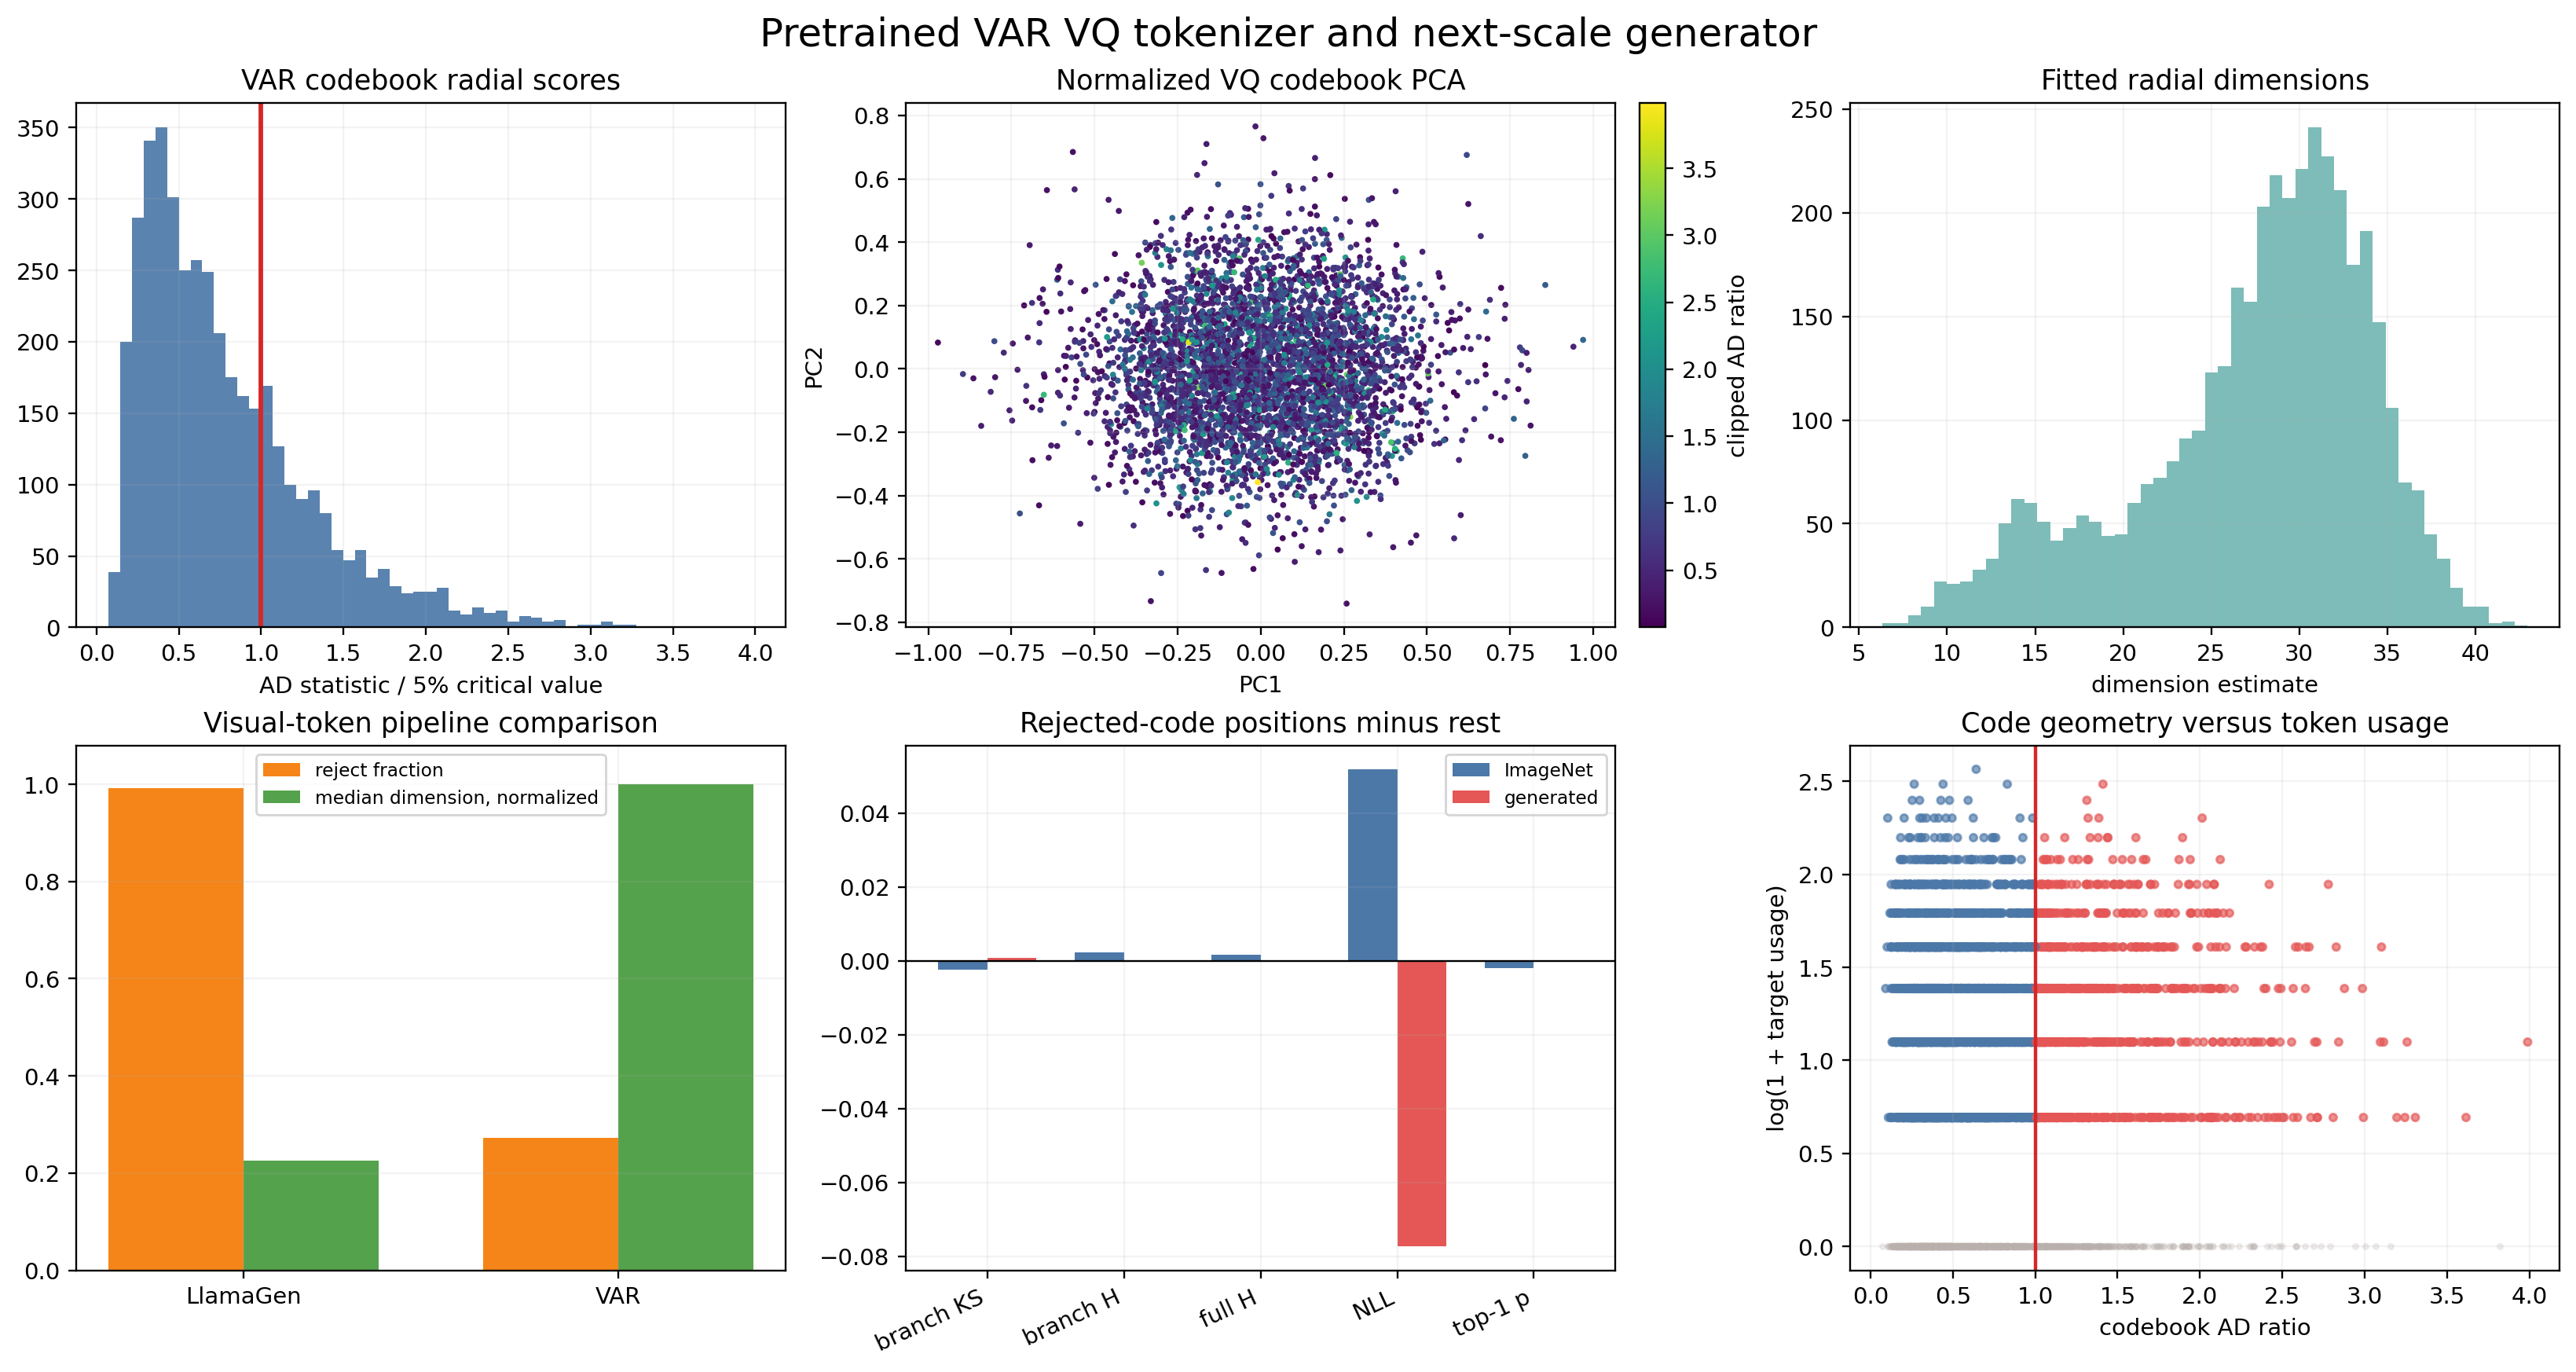
\includegraphics[width=0.95\linewidth]{images/var_shell_dashboard.png}
\caption{VAR-d16 experiment summary. The normalized VAR codebook has a much
lower shell-test rejection rate than the normalized LlamaGen codebook, while
image-level generator associations remain small and uncertain.}
\label{fig:var-dashboard}
\end{figure}

\begin{figure}[p]
\centering
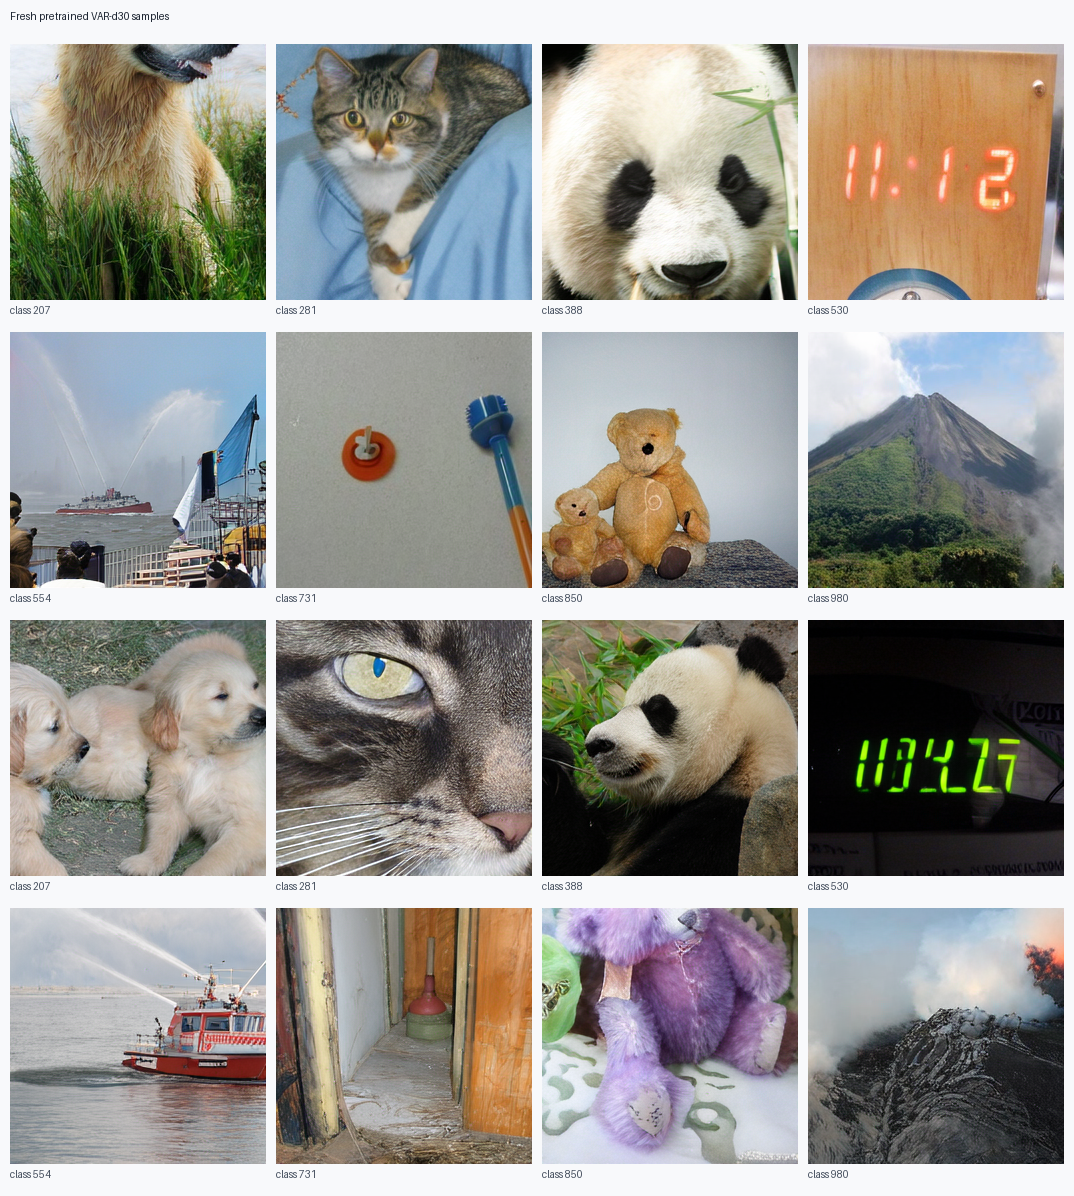
\includegraphics[width=0.95\linewidth]{images/var_generated_samples.png}
\caption{Class-conditional $256\times256$ samples generated by the released
VAR-d30 pipeline and used in the generated-image experiment.}
\label{fig:var-samples}
\end{figure}

\begin{figure}[p]
\centering
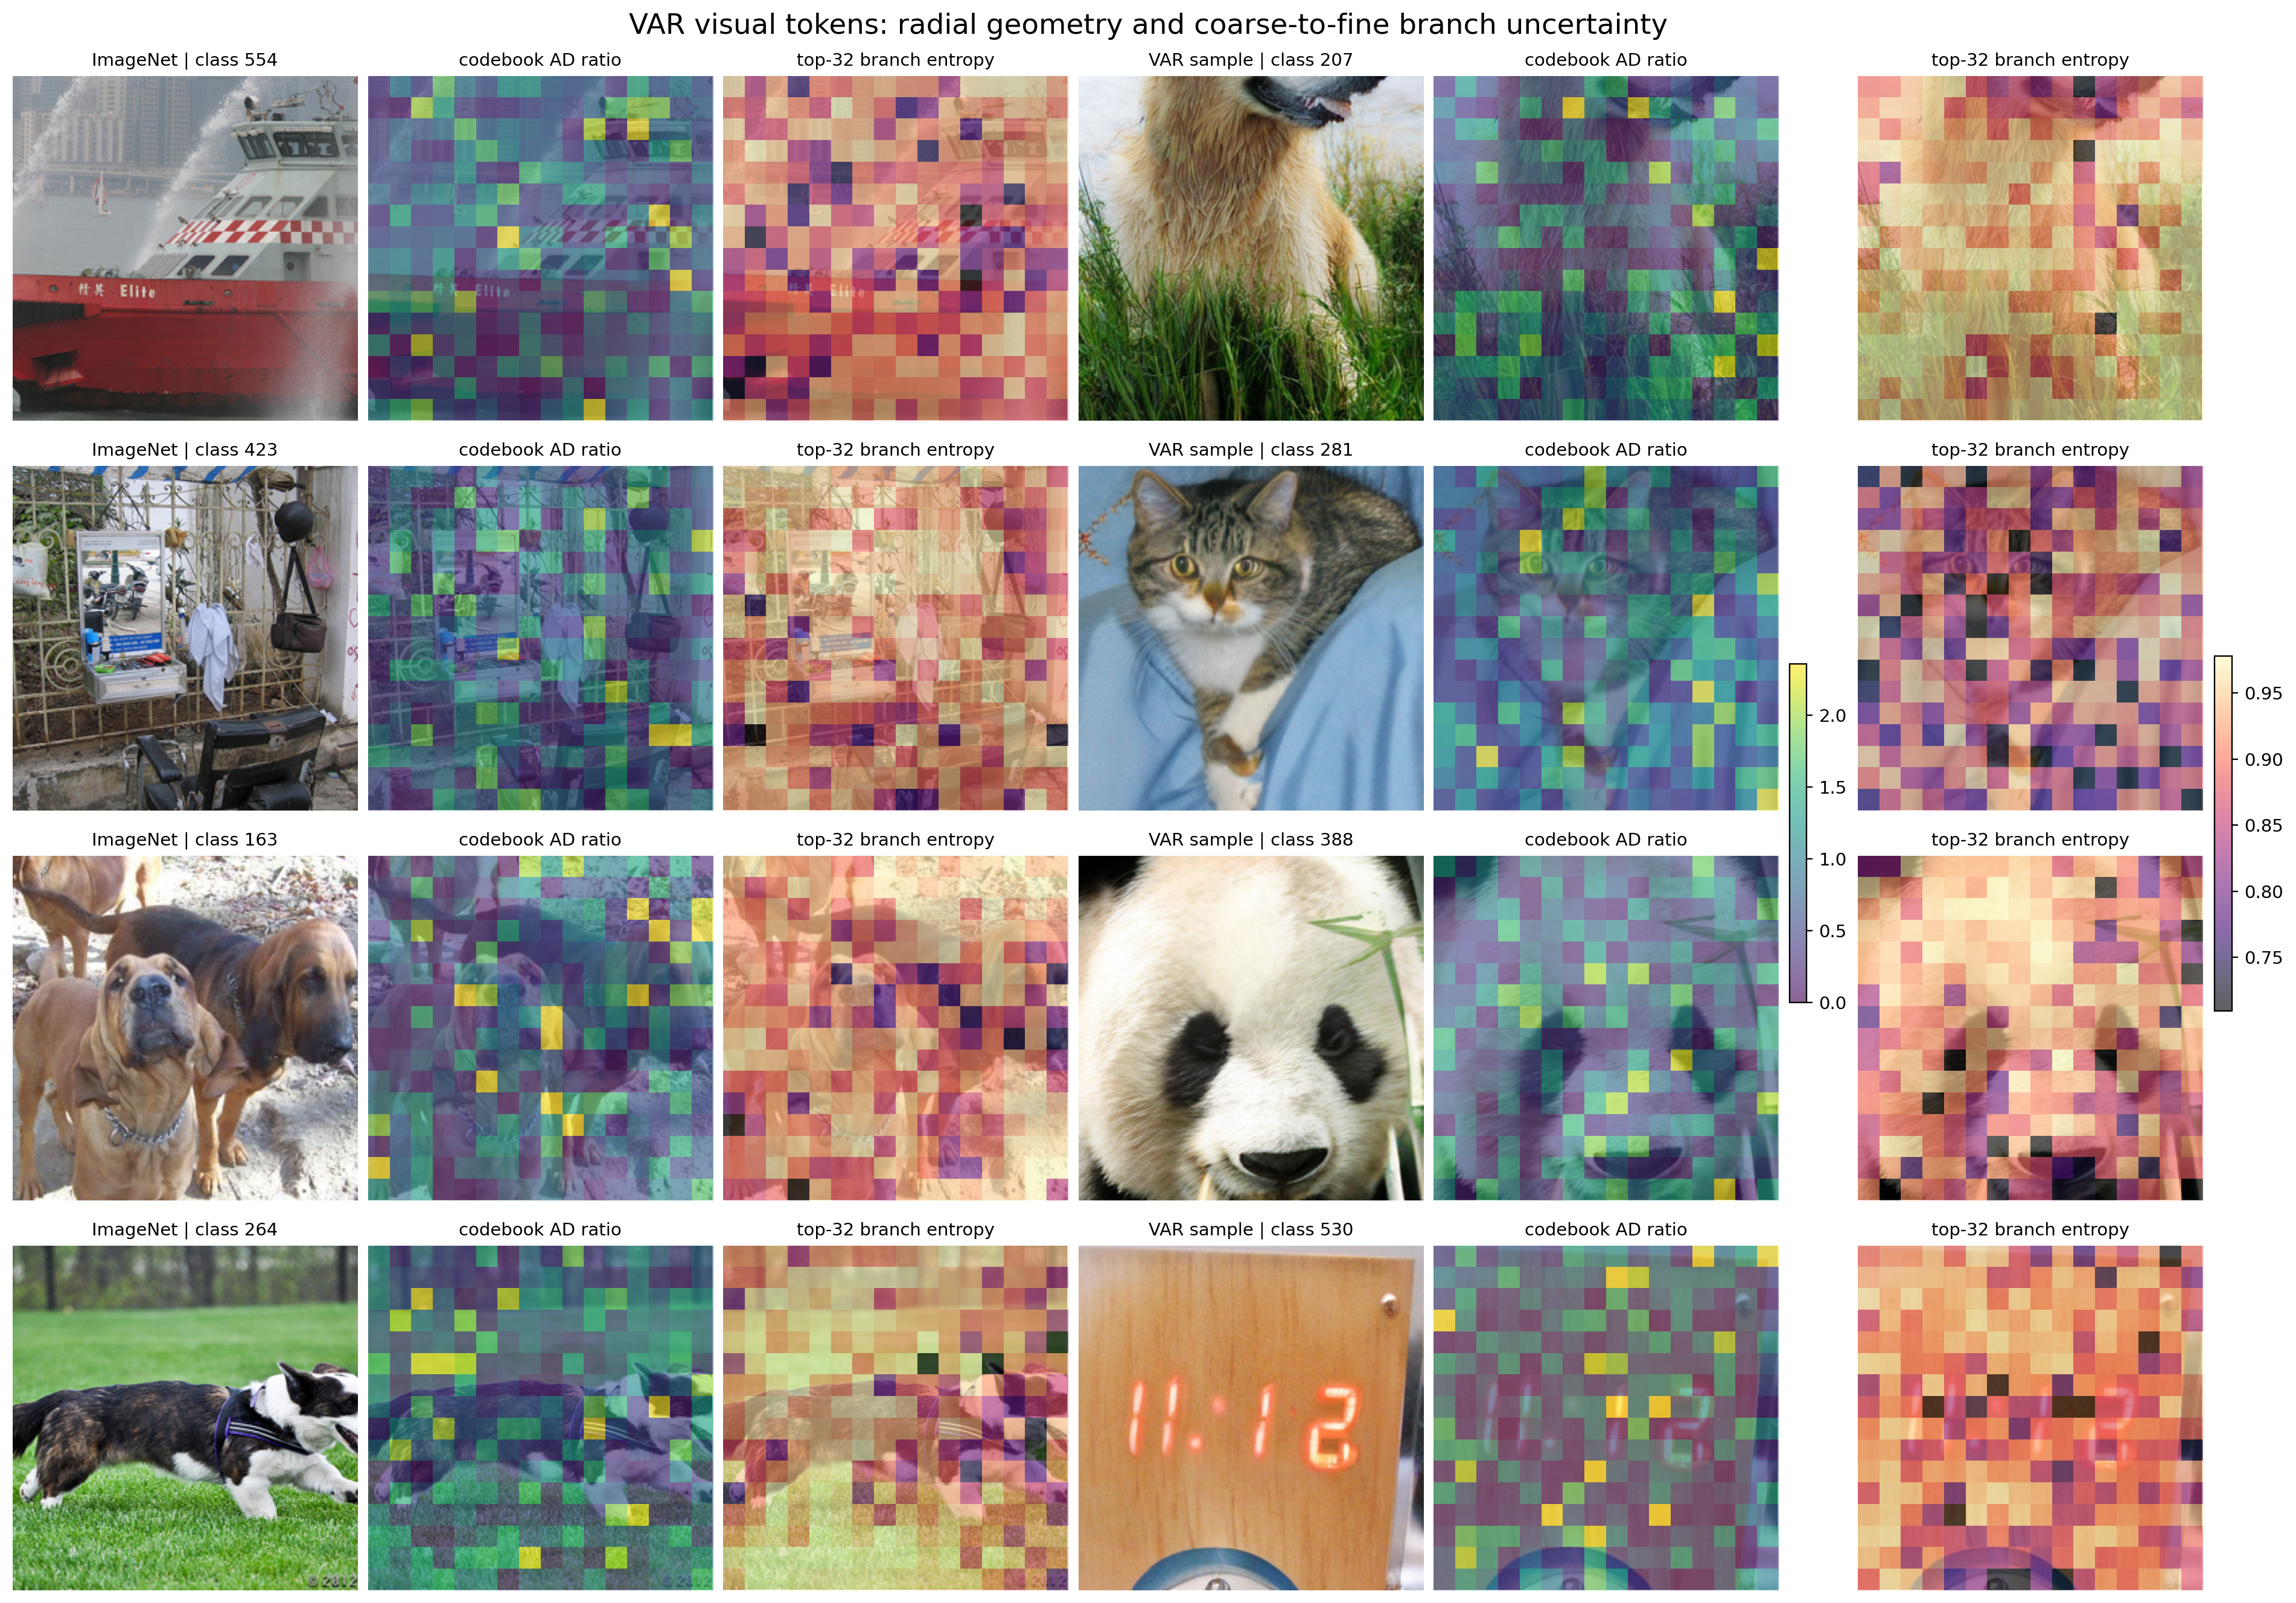
\includegraphics[width=0.95\linewidth]{images/var_imagenet_generated_shell_gallery.png}
\caption{VAR-d30 spatial diagnostics for real ImageNet inputs and generated
images. Each row shows the image, the normalized Anderson--Darling score of its
target codes, and normalized entropy among the top-32 predicted codes.}
\label{fig:var-heatmaps}
\end{figure}

\section{Interpretation and Limitations}

The argument has a deliberate logical hierarchy:
\[
  \begin{aligned}
    &\text{local Euclidean topology}\\[-0.2em]
    &\quad+\ \text{local metric regularity}\\[-0.2em]
    &\quad+\ \text{local volume-uniform sampling}\\
    &\hspace{3em}\Longrightarrow\ \text{radial volume law}.
  \end{aligned}
\]
The test examines only the conclusion on the right. A rejection is evidence
against the radial law at the selected scale, and therefore against the full
conjunction of assumptions. It does not identify whether topology, metric
regularity, or sampling density caused the failure. Conversely, a
non-rejection only means that this particular radial signature was not
distinguished from the reference law with the available neighborhood.

\subsection{Empirical Synthesis}

The controlled experiments first establish that the decision rule behaves as
intended: its null rejection rate remains close to the nominal $5\%$ level, and
its power rises against both inner-heavy and outer-heavy radial alternatives.
The empirical rejection rates are therefore interpretable as genuine failures
of the localized smooth-volume model rather than an obvious calibration
artifact.

\begin{table}[H]
\centering
\small
\caption{Cross-representation synthesis. Rejection rates measure failure of
the exact local radial-volume law, not the prevalence of topological
singularities.}
\begin{tabular}{@{}>{\raggedright\arraybackslash}p{0.23\linewidth}>{\raggedright\arraybackslash}p{0.19\linewidth}>{\raggedright\arraybackslash}p{0.14\linewidth}>{\raggedright\arraybackslash}p{0.31\linewidth}@{}}
\toprule
Representation & Tested unit & Result & Supported interpretation \\
\midrule
ImageNet patch features & 3136 patch anchors & $44.52\%$ reject & Spatially heterogeneous radial geometry \\
LlamaGen VQ codebook & 16384 normalized codes & $99.16\%$ reject & Prototype spacing strongly mismatches the null \\
VAR VQ codebook & 4096 normalized codes & $27.29\%$ reject & Strong tokenizer dependence \\
VAR-d16/d30 generator & Four groups of 16 images & no $p<0.05$ & No reliable branch-uncertainty association \\
\bottomrule
\end{tabular}
\label{tab:synthesis}
\end{table}

The combined result is evidence against a universal model in which all vision
tokens inhabit one locally homogeneous, uniformly sampled manifold. Local
radial behavior varies across image positions and differs sharply between two
released tokenizers. This representation dependence is itself part of the
scientific result: ``visual-token geometry'' is not invariant to the tokenizer,
embedding dimension, normalization, training objective, or neighborhood rule.

\subsection{Relation to the Stratified Manifold Hypothesis}

The observations are compatible with a stratified picture. In such a picture,
anchors in the interior of a regular stratum should approximately follow one
local dimension and may satisfy the volume law at an appropriate scale. Points
near a boundary, an intersection of strata, or a mixture of semantic regimes
may instead show distorted radial growth and reject. The ImageNet heatmaps,
which often highlight texture transitions, repeated structure, and object or
background boundaries, qualitatively fit this account.

Compatibility is not proof. Nonuniform density, anisotropic covariance,
curvature, quantization, metric distortion, duplicate representations, and
overlapping neighborhoods can all produce the same radial rejection without
changing local topology. Likewise, a distribution can have the correct radial
law while concentrating in a small set of angular directions. The present
results therefore support the weaker statement that vision representations
have heterogeneous local measure geometry, one possible explanation of which
is stratification.

A stronger stratification result would require several signatures to occur
together: approximately stable local dimension within candidate strata,
persistent rejection near reproducible boundaries across neighborhood scales,
dimension changes across those boundaries, regular tangent or angular geometry
inside strata, and direct topological evidence such as stable local homology.
These properties should replicate across images, datasets, model seeds, and
semantically equivalent inputs.

\subsection{Tokenizer Geometry and Generator Behavior}

The LlamaGen and VAR comparisons separate a static geometric object from a
conditional probabilistic object. A VQ codebook is a finite learned dictionary
of prototypes. A generator posterior is a context-dependent distribution over
that dictionary. Consequently,
\[
  \text{irregular codebook geometry}
  \quad\not\Longrightarrow\quad
  \text{uncertain generator prediction}.
\]
The LlamaGen shifts are exploratory because $98.47\%$ of joined positions use
rejected target codes, leaving only 250 non-rejected positions for comparison.
For VAR, none of the four image-level comparisons reaches $p<0.05$, and the
association does not strengthen from d16 to d30. Thus codebook rejection alone
does not establish polysemy, multimodality, or branching in the generator.

\subsection{Scope of the Statistical Claim}

The fitted-scale Anderson--Darling test is a diagnostic of exact radial shape,
not an equivalence test for approximate uniformity. Formally certifying that a
neighborhood lies within a prescribed tolerance would require a confidence
bound or an equivalence procedure for the selected discrepancy. Decisions are
also dependent when nearby anchors share neighbors, so any global discovery
claim should include an appropriate multiple-testing method and sensitivity to
neighborhood size.

A fuller geometric assessment can combine the radial statistic with an angular
test on normalized directions $(X_i-t)/\|X_i-t\|_2$, or first estimate and
whiten local tangent coordinates before testing radius and direction. Future
generator experiments should test occupancy-weighted encoder states and hidden
representations in addition to codebook prototypes, and should include masked
or discrete-diffusion visual-token generators whose conditioning mechanisms
differ from raster-order and next-scale autoregression.

\section{Summary}

The global hypothesis states that every token $t\in\mathcal E$ admits a radius
$r_\ast(t)$ for which its open neighborhood in the representation support is
homeomorphic to $\R^{d(t)}$. Since homeomorphism alone determines neither
distances nor probabilities, the testable localized hypothesis additionally
assumes approximately Euclidean metric geometry and uniform sampling with
respect to intrinsic volume.

For an anchor $t$, retain neighboring representations inside radius $r_\ast$.
Under the resulting locally uniform $d$-dimensional tangent-ball model,
\[
  \Prb(\|X-t\|_2\le r\mid \|X-t\|_2\le r_\ast)
  =\left(\frac{r}{r_\ast}\right)^d.
\]
Thus the shell index has PMF
\[
  q_k(d)=\frac{r_k^d-r_{k-1}^d}{r_\ast^d},
\]
which becomes uniform, $q_k=1/K$, when the boundaries define equal-volume
shells. This is the discrete, visual version of the localized hypothesis.
Consequently $Z=\log(r_\ast/\|X-t\|_2)$ is exponential with unknown rate $d$.
We estimate $d=1/\overline Z$, standardize the log-radii by their mean, and use
the Anderson--Darling statistic to test exponential shape. The decision compares
$A_N^2$ with a fitted-scale critical value, and rejection identifies anchors
whose radial mass growth is inconsistent with the simplest local smooth-volume
model.

\section{Conclusion}

The proposed stratified manifold hypothesis is topological, while our test
targets a necessary measure-geometric consequence: intrinsic-volume growth in
a regular neighborhood. Under local uniformity this growth yields an
exponential log-radius law, which the fitted-scale Anderson--Darling statistic
tests with calibrated finite-sample critical values.

The experiments reject a universal locally homogeneous account of vision-token
space: ImageNet patches reject at $44.52\%$, while normalized LlamaGen and VAR
codebooks reject at $99.16\%$ and $27.29\%$. This architecture- and
location-dependent heterogeneity is compatible with stratification, but radial
rejection can also result from density, anisotropy, curvature, quantization, or
metric distortion. Finite codebooks are therefore geometric proxies for latent
supports, not literal positive-dimensional manifolds.

The VAR results further show that tokenizer geometry does not imply generator
uncertainty. The strongest supported conclusion is that vision representations
have heterogeneous local measure geometry. Establishing stratification itself
requires aligned evidence from stable local dimensions, tangent and angular
regularity, scale-persistent boundaries, and direct topological diagnostics.

\begin{thebibliography}{9}
\small
\setlength{\itemsep}{0.25em}

\bibitem{sun2024llamagen}
Peize Sun, Yi Jiang, Shoufa Chen, Shilong Zhang, Bingyue Peng, Ping Luo, and
Zehuan Yuan.
\newblock Autoregressive Model Beats Diffusion: Llama for Scalable Image
Generation.
\newblock arXiv:2406.06525, 2024.

\bibitem{tian2024var}
Keyu Tian, Yi Jiang, Zehuan Yuan, Bingyue Peng, and Liwei Wang.
\newblock Visual Autoregressive Modeling: Scalable Image Generation via
Next-Scale Prediction.
\newblock Advances in Neural Information Processing Systems, 2024.

\end{thebibliography}

\end{document}
